\documentclass[answers]{exam}

\usepackage{amsmath}
\usepackage{amssymb}
\usepackage{geometry}
\usepackage{venndiagram}
\usepackage{graphics}
\usepackage{graphicx}
\usepackage{tikz}

% Header and footer.
\pagestyle{headandfoot}
\runningheadrule
\runningfootrule
\runningheader{MATH 402 Applied Stochastic Processes}{Assignment 1}{Fall 2023}
\runningfooter{}{Page \thepage\ of \numpages}{}
\firstpageheader{}{}{}

\boxedpoints
\printanswers

\newcommand{\uvec}[1]{\boldsymbol{\hat{\textbf{#1}}}}
\newcommand\union\cup
\newcommand\inter\cap
\newcommand\ul\underline
\newcommand\ol\overline

\title{Homework 1\\ MATH 402 Applied Stochastic Processes\\ Habib University -- Fall 2023}
\author{Ali Asghar Yousuf \\ ay06993}  % replace with your ID, e.g. oy02945
\date{\today}

\begin{document}
\maketitle

\begin{questions}
    \question A number $U$ is selected at random from the unit interval. Let the events $A$ and $B$ be:
    $A$ = ``$U$ differs from $\frac{1}{2}$ by more than $\frac{1}{4}$'' and $B$ = ``$1 - U$ is less than $\frac{1}{2}$.''
    Find the events:
    \begin{parts}
        \part $A \cap B$
        \begin{solution}
            \(A \cap B = \left\{U \in [0, 1] \mid \left| U - \frac{1}{2} \right| > \frac{1}{4} \text{ and } 1 - U < \frac{1}{2}\right\}\)

        \end{solution}
        \part $A \cup B$
        \begin{solution}
            \(A \cup B = \left\{U \in [0, 1] \mid \left| U - \frac{1}{2} \right| > \frac{1}{4} \text{ or } 1 - U < \frac{1}{2}\right\}\)

        \end{solution}
        \part $A^c \cap B$
        \begin{solution}
            \(A^c \cap B = \left\{U \in [0, 1] \mid \left| U - \frac{1}{2} \right| \leq \frac{1}{4} \text{ and } 1 - U < \frac{1}{2}\right\}\)

        \end{solution}
    \end{parts}

    \question Let $A, B,$ and $C$ be events. Find expressions for the events:
    \begin{parts}
        \part Exactly one of the three events occurs.
        \begin{solution}
            \((A \cap B' \cap C') \cup (A' \cap B \cap C') \cup (A' \cap B' \cap C)\)

        \end{solution}
        \part Exactly two of the events occur.
        \begin{solution}
            \((A \cap B \cap C') \cup (A \cap B' \cap C) \cup (A' \cap B \cap C)\)

        \end{solution}
        \part One or more of the events occur.
        \begin{solution}
            \(A \cup B \cup C\)

        \end{solution}
        \part Two or more of the events occur.
        \begin{solution}
            \((A \cap B) \cup (A \cap C) \cup (B \cap C) \cup (A \cap B \cap C)\)

        \end{solution}
        \part None of the events occur.
        \begin{solution}
            \(A' \cap B' \cap C'\)

        \end{solution}
    \end{parts}

    \question In a specified 8-AM-to-8-AM 24-hour period, a student wakes up at time $t_1$  and goes to sleep at some later time $t_2$.
    \begin{parts}
        \part
        Find the sample space and sketch it on the x-y plane if the outcome of this experiment consists of the pair $(t_1, t_2)$
        \begin{solution}
            The sample space for this experiment consists of all possible pairs of times $(t_1, t_2)$ when the student wakes up at time $t_1$ and goes to sleep at time $t_2$. Since it's a 24-hour period, both $t_1$ and $t_2$ can range from 0 (midnight) to 24 (midnight of the next day). However, $t_2$ should be greater than or equal to $t_1$ since the student goes to sleep after waking up.

            So, the sample space is the set of all pairs $(t_1, t_2)$ where $0 \leq t_1
                \leq 24$ and $t_1 \leq t_2 \leq 24$.

            The sample space for this experiment is the triangle shown in the figure below.

            \begin{center}
                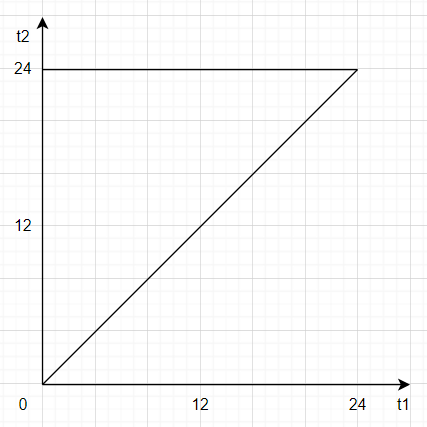
\includegraphics[width=0.5\textwidth]{images/3a.png}
            \end{center}

        \end{solution}
        \part
        Specify the set $A$ and sketch the region on the plane corresponding to the event “student is asleep at noon.”
        \begin{solution}
            The event “student is asleep at noon” corresponds to when the student wakes up after noon or wakes up before noon and goes to sleep before noon as well. The set of all pairs $(t_1, t_2)$ where $4 < t_1 < t_2$ or $t_1 < t_2 < 4$.
            The set $A$ is the shaded region in the figure below.

            \begin{center}
                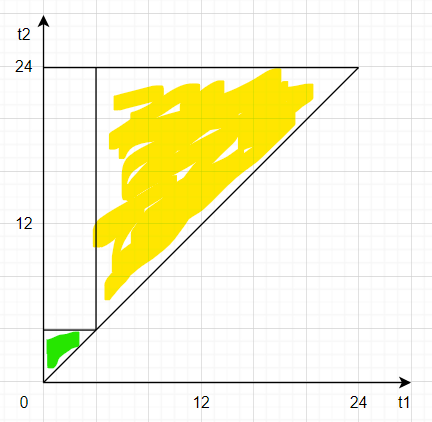
\includegraphics[width=0.5\textwidth]{images/3b.png}
            \end{center}

            The yellow shaded region corresponds to the set $4 < t_1 < t_2$ and the green
            shaded region corresponds to the set $t_1 < t_2 < 4$, and the union of these
            two regions is the set $A$.

        \end{solution}
        \part
        Specify the set $B$ and sketch the region on the plane corresponding to the event “student sleeps through breakfast (9–10 AM).”
        \begin{solution}
            The event “student sleeps through breakfast (9-10 AM)” corresponds to when the student wakes up after 10 AM or wakes up before 9 AM and goes to sleep before 9 AM as well. The set of all pairs $(t_1, t_2)$ where $2 < t_1 < t_2$ or $t_1 < t_2 < 1$.
            The set $B$ is the shaded region in the figure below.

            \begin{center}
                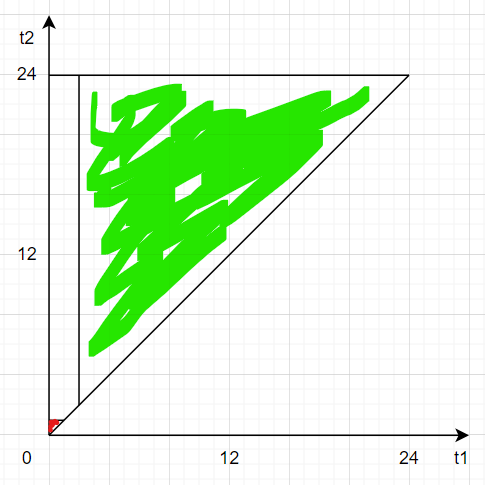
\includegraphics[width=0.5\textwidth]{images/3c.png}
            \end{center}

            The green shaded region corresponds to the set $2 < t_1 < t_2$ and the red
            shaded region corresponds to the set $t_1 < t_2 < 1$, and the union of these
            two regions is the set $B$.
        \end{solution}
        \part Sketch the region corresponding to $A \cap B$ and describe the corresponding event in words.
        \begin{solution}
            The set $A \cap B$ is the intersection of the sets $A$ and $B$ where the student wakes up after noon or wakes up before 9 AM and goes to sleep before 9 AM as well.
            The set $A \cap B$ is the set of all pairs $(t_1, t_2)$ where $4 < t_1 < t_2$ or $t_1 < t_2 < 1$.
            The set $A \cap B$ is the shaded region in the figure below.

            \begin{center}
                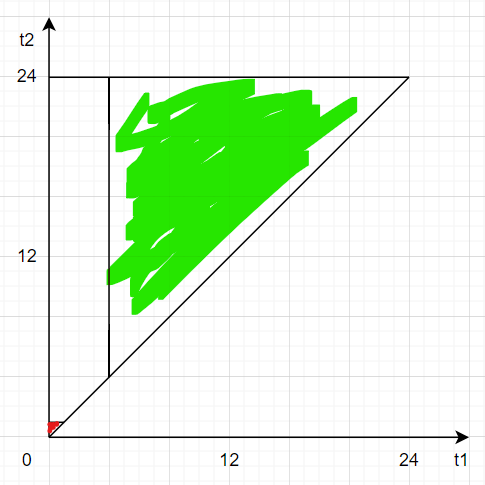
\includegraphics[width=0.5\textwidth]{images/3d.png}
            \end{center}

            The green shaded region corresponds to the set $4 < t_1 < t_2$ and the red
            shaded region corresponds to the set $t_1 < t_2 < 1$, and the union of
            these two regions is the set $A \cap B$.
        \end{solution}
    \end{parts}

    \question
    A dart is equally likely to land at any point inside a circular target of radius 2. Let $R$ be the distance of the landing point from the origin.
    \begin{parts}

        \part
        Find the sample space $S$ and the range if $R$, $S_R$;

        \part
        Show the mapping from $S$ to $S_R$;

        \part
        The ``bull's eye'' is the central disk in the target of radius 0.25. Find the event $A$ in $S_R$ corresponding to ``dart hits the bull's eye.'' Find the equivalent event in S and $P(A)$.

        \part
        Find and plot the cdf of $R$.
    \end{parts}

    \newpage

    \question
    A voltage $X$ is uniformly distributed in the set $\{-3, -2, \dots, 3, 4\}$.
    \begin{parts}

        \part Find the mean and variance of $X$.
        \part Find the mean and variance of $Y = -2 X^22 + 3$.
        \part Find the mean and variance of $Z = \cos (\pi X/8)$.
        \part Find the mean and variance of $W = \cos^2  (\pi X/8)$.
    \end{parts}

    \question
    A random variable $X$ has pdf:
    \begin{equation*}
        f_X(x) = \begin{cases}
            c x (1 - x^2), & 0 \le x \le 1,    \\
            0,             & \text{elsewhere}.
        \end{cases}
    \end{equation*}
    \begin{parts}

        \part Find c and plot the pdf and the cdf of X.
        \part Find $P(0 \le X \le 0.5)$, $P(X = 1)$, and $P(0.25 \le X \le 0.5)$.
    \end{parts}

    \question
    Consider two RVs, X and Y, and an RV, Z, such that $P[Z = X] = p$ and $P[Z = Y] = 1 - p$.

    \begin{parts}

        \part Show that the pdf of Z is given by
        $$
            f_Z(z) = p f_X(z) + (1-p) f_Y(z).
        $$
        \part Calculate the cdf of two-sided exponential RV that has PDF given by
        \begin{equation*}
            f_Z(z) = \begin{cases}
                p \lambda e^{\lambda z},        & z < 0,   \\
                (1 - p) \lambda e^{-\lambda z}, & z \ge 0.
            \end{cases}
        \end{equation*}
        where $\lambda > 0$ and $0 < p < 1$.
    \end{parts}
\end{questions}

\end{document}